\documentclass[11pt]{article}

\usepackage[a4paper,margin=1in]{geometry}
\usepackage[T1]{fontenc}
\usepackage[utf8]{inputenc}
\usepackage{lmodern}
\usepackage{graphicx}
\usepackage{hyperref}
\usepackage{amsmath}

\hypersetup{
  colorlinks=true,
  linkcolor=black,
  urlcolor=blue,
  pdftitle={Stability Oracle v1 Main Paper},
  pdfauthor={OpenAI Codex},
  pdfsubject={Stability Oracle main reference paper}
}
\setcounter{secnumdepth}{3}
\setcounter{tocdepth}{2}

\title{Stability Oracle v1\\Main Reference Paper}
\author{Frozen Reference Release}
\date{March 25, 2026}

\begin{document}
\maketitle
\tableofcontents
\newpage

\section{Purpose}

This paper records the frozen v1 reference state of Stability Oracle.

The project is intentionally small.
It exposes one bounded capability:

\begin{quote}
Given a structured state or trajectory representation, determine whether meaningful organization remains recoverably coherent under change.
\end{quote}

This is not a physics engine, robotics stack, or cognition model.
It is a deterministic structural stability instrument.

\section{Operational Scope}

The oracle answers one operational question:

\begin{quote}
Does a configuration remain structurally survivable when perturbed or evolved?
\end{quote}

The engine is designed to be:

\begin{itemize}
\item deterministic
\item bounded
\item reproducible
\item modular
\item agent-callable
\end{itemize}

The project does not claim ontology, consciousness modeling, or universal semantics.
It only evaluates structural persistence under change.

\section{Core Contract}

The v1 kernel is built around a compact typed contract:

\begin{itemize}
\item \texttt{State}: minimal structural state representation
\item \texttt{Perturbation}: bounded structural disturbance description
\item \texttt{StabilityMetrics}: deterministic metric bundle
\item \texttt{OracleResult}: bounded machine-readable outcome
\end{itemize}

The public output surface contains:

\begin{itemize}
\item classification
\item structural retention
\item temporal consistency
\item causal deformation
\item geometric integrity
\item confidence
\item coherence score
\item policy version
\item short summary
\end{itemize}

\section{Architecture}

The frozen v1 architecture is layered:

\begin{enumerate}
\item state and perturbation language layer
\item pluggable metric layer
\item deterministic policy classifier
\item Oracle Engine v2
\item deterministic routing layer
\item telemetry ingestion layer
\item public demo and documentation surfaces
\end{enumerate}

The execution kernel remains the logical oracle.
The telemetry layer is parallel to it, not a rewrite of it.

\begin{figure}[h]
  \centering
  \includegraphics[width=\textwidth]{../../docs/assets/stability-oracle-evaluation-layer-overview.png}
  \caption{Frozen Stability Oracle evaluation-layer view.}
\end{figure}

\section{Metric and Policy Surface}

The metric surface is deliberately minimal and deterministic.
The four invariant metrics are:

\begin{itemize}
\item structural retention
\item temporal consistency
\item causal deformation
\item geometric integrity
\end{itemize}

The classifier normalizes polarity, applies a survivability floor, computes coherence and spread, and returns one of:

\begin{itemize}
\item stable
\item marginal
\item unstable
\end{itemize}

The default policy version is:

\begin{verbatim}
v1_floor_mean_band
\end{verbatim}

This keeps classification transparent and calibration-friendly without learned weights or hidden heuristics.

\section{Oracle Engine and Router}

Oracle Engine v2 provides three deterministic paths:

\begin{itemize}
\item transition evaluation
\item perturbation evaluation
\item batch scanning
\end{itemize}

The routing layer adds explicit domain selection labels:

\begin{itemize}
\item LOGICAL
\item PHYSICAL
\item FOUNDATIONAL
\item UNKNOWN
\end{itemize}

Only LOGICAL is implemented in v1.
The other route labels return bounded stubs rather than pretending to exist.

\section{Telemetry Decoupling}

The key v1 decoupling move is the telemetry layer.
It introduces:

\begin{itemize}
\item \texttt{TelemetryFrame}
\item \texttt{TelemetrySequence}
\item deterministic validation
\item deterministic normalization
\item deterministic geometry encoding
\item a narrow telemetry bridge back into the logical kernel
\end{itemize}

This layer allows foreign domains to be expressed as fixed-width telemetry without changing oracle semantics.

The critical migration rule is:

\begin{quote}
Prove parity on HAOS-shaped inputs first, then generalize.
\end{quote}

\section{Public Demonstrations}

The frozen v1 state includes two public non-trivial demonstrations.

\subsection{LLM Reasoning Telemetry}

The first demo treats stepwise reasoning traces as fixed-width telemetry.

Frozen characteristics:

\begin{itemize}
\item 12 traces
\item 8-dimensional telemetry
\item coherent $\rightarrow$ stable
\item drifted $\rightarrow$ marginal
\item broken $\rightarrow$ unstable
\end{itemize}

This demo shows that the oracle can detect structural reasoning drift using only trajectory geometry.

\begin{figure}[h]
  \centering
  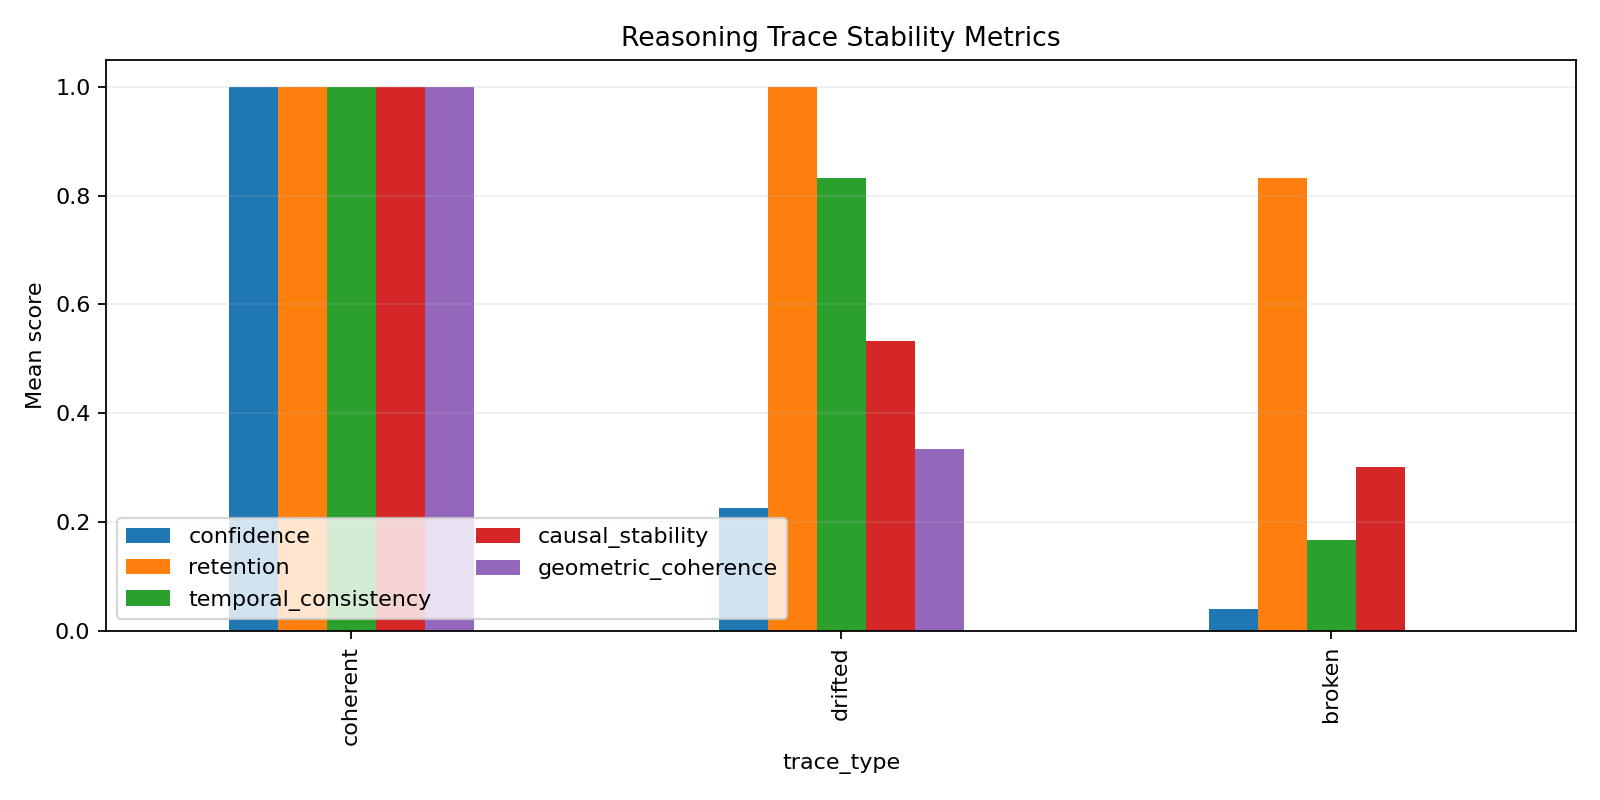
\includegraphics[width=\textwidth]{../../docs/assets/llm-reasoning-demo-metrics-plot.png}
  \caption{LLM reasoning telemetry demo metric separation.}
\end{figure}

\subsection{Continuous Agent Trajectory Stability}

The second demo uses continuous 2-D point-agent trajectories with damped goal-seeking dynamics.

Frozen characteristics:

\begin{itemize}
\item 15 trajectories
\item 8-dimensional telemetry
\item stable $\rightarrow$ stable
\item marginal $\rightarrow$ marginal
\item unstable $\rightarrow$ unstable
\end{itemize}

This demo matters because it is geometrically continuous rather than symbolic and discrete.
It shows that the same oracle can classify structural quality in both domains through the same kernel.

\begin{figure}[h]
  \centering
  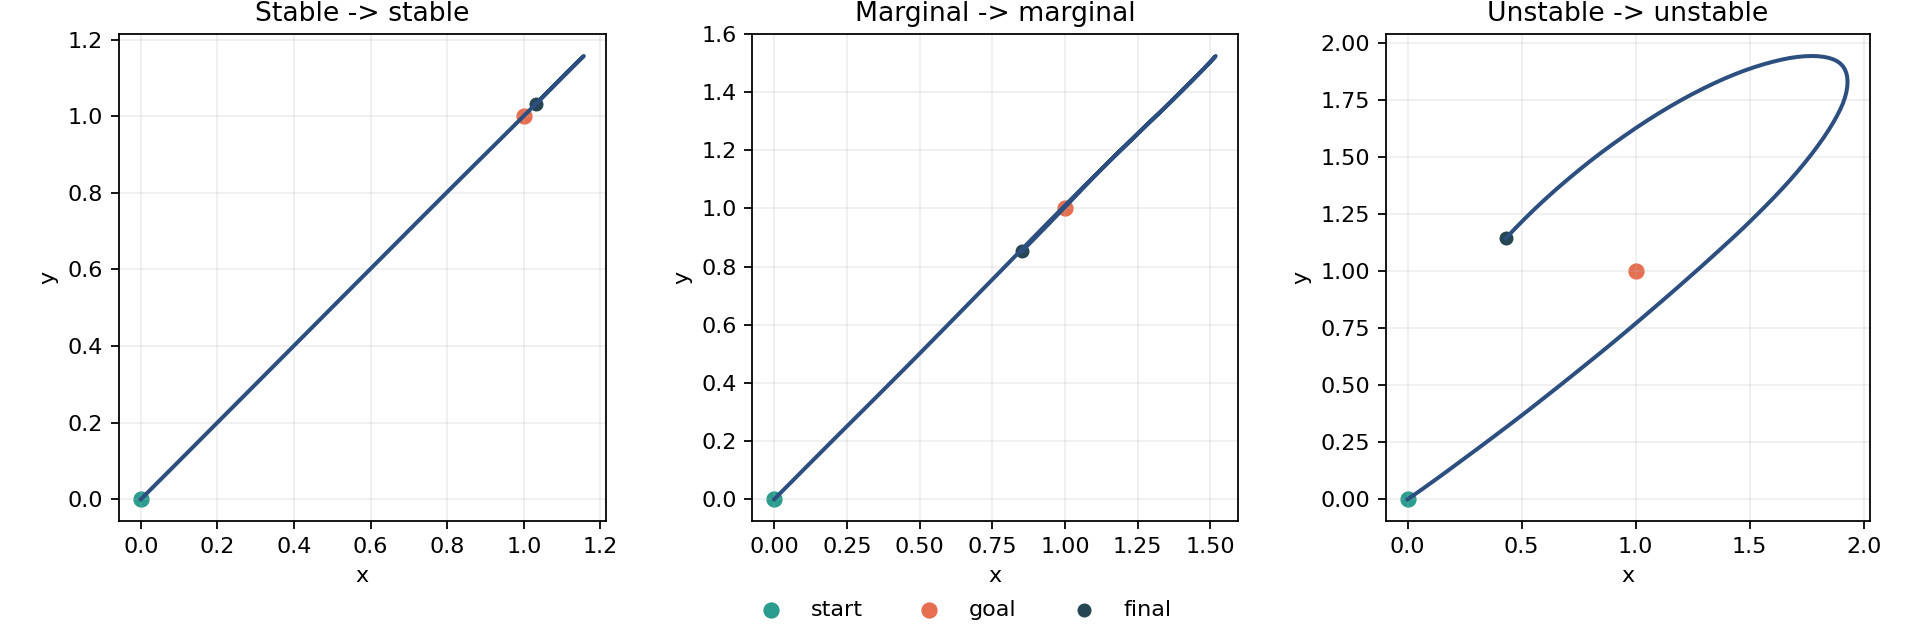
\includegraphics[width=\textwidth]{../../docs/assets/agent-trajectory-demo-plot.png}
  \caption{Continuous agent trajectory demo with stable, marginal, and unstable paths.}
\end{figure}

\section{Design Guarantees}

The frozen v1 reference implementation guarantees:

\begin{itemize}
\item deterministic evaluation
\item bounded JSON output
\item no stochastic classification logic
\item no filesystem writes by default in the core package
\item read-only separation from research artifacts
\item fail-closed validation behavior
\end{itemize}

\section{Project Status}

The project is now frozen as a reference artifact.

Current status:

\begin{itemize}
\item development paused
\item engine considered stable reference implementation
\item future work exploratory only
\end{itemize}

No further changes are planned unless they address:

\begin{itemize}
\item a bug
\item broken reproducibility
\item a documentation typo
\end{itemize}

\section{Conclusion}

Stability Oracle v1 is complete at the right scale.

It now exists as:

\begin{itemize}
\item a deterministic structural stability engine
\item a telemetry-ingestible logical kernel
\item a reproducible reference implementation
\item a public artifact with two cross-domain demonstrations
\end{itemize}

The value of the project is not in breadth.
It is in having a small instrument that is clear, reproducible, and operationally honest.

\end{document}
